
\chapter{Ugeopgave 9}
\label{cha:ugeopgave-9}

\section{Part 2}

Vi reflekterer thepotten i vores plan der indeholder vores ``quad''. Vi skal spejle billedet ved at skifte orienteringen.

\section{Part 3}

Dern�st skal der ops�ttes endnu en lyskilde som bruges n�r vi tegner reflektionen.

\section{Part 4}

Vi sikrer os at draw_mirror kaldes f�r draw_proj_shadow i display funktionen. draw_proj_shadow p�virker farve bufferen og denne skal derfor sl�es fra og til f�r og efter funktionen kaldes. Texturplanet skal blendes med reflektionen af thepotten. Resultatet kan ses i figur \ref{fig:9-1-1}.

\begin{figure}[hp]
\centering
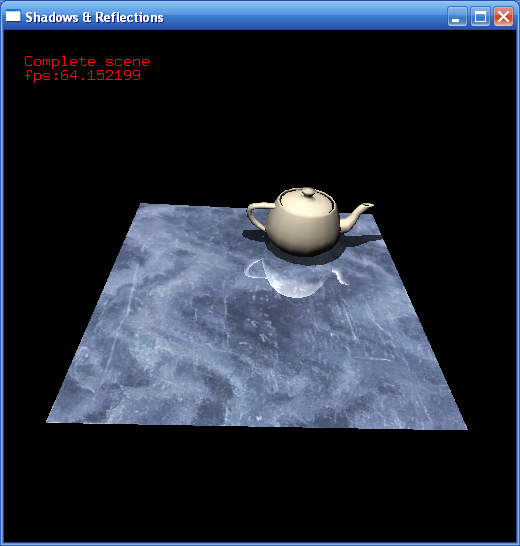
\includegraphics[width=8cm]{../exercise9/screenshots/4.png}
\caption{Thekande}
\label{fig:9-1-1}
\end{figure}

\section{Part 5}

For at rette op p� en mindre fejl, at der kan blivee tegnet reflektion uden for reflektionsplanet, tegner vi f�rst reflektionsplanet. N�r reflektionen s� skal tegnes bruger vi vores stencil buffer og tegner derved kun reflektionen steder hvor der allerede er tegnet. Derved undg�r vi at tegne uden for vores ``quad''


\section{Part 6}

Der st�r i opgaven at man skal lade thepotten g� igennem vores ``quad''. Det har den nu gjort siden part 1 i exercise09. Derved opst�r der ikke noget nyt problem da vi allerede har taget h�jde for dette med et clipping plane som vi introducerede i exercise08.


